\begin{fact} \label{tri-one-side-fixed}
	Considérons tous les triangles de périmètre fixé, et ayant tous un côté en commun.
	Parmi tous ces triangles, un seul est d'aire maximale, c'est le triangle isocèle ayant pour base le côté commun.
\end{fact}


\begin{proof}
	Soit $ABC$ un triangle de périmètre $p$, et fixons le côté $[AB]$. 
	Pour tout point $M$ sur la parallèle à $(AB)$ passant par $C$, nous savons que $\area{ABM} = \area{ABC}$. Notons alors $O$ le point sur cette parallèle tel que $ABO$ soit isocèle en $O$.

	\begin{center}
		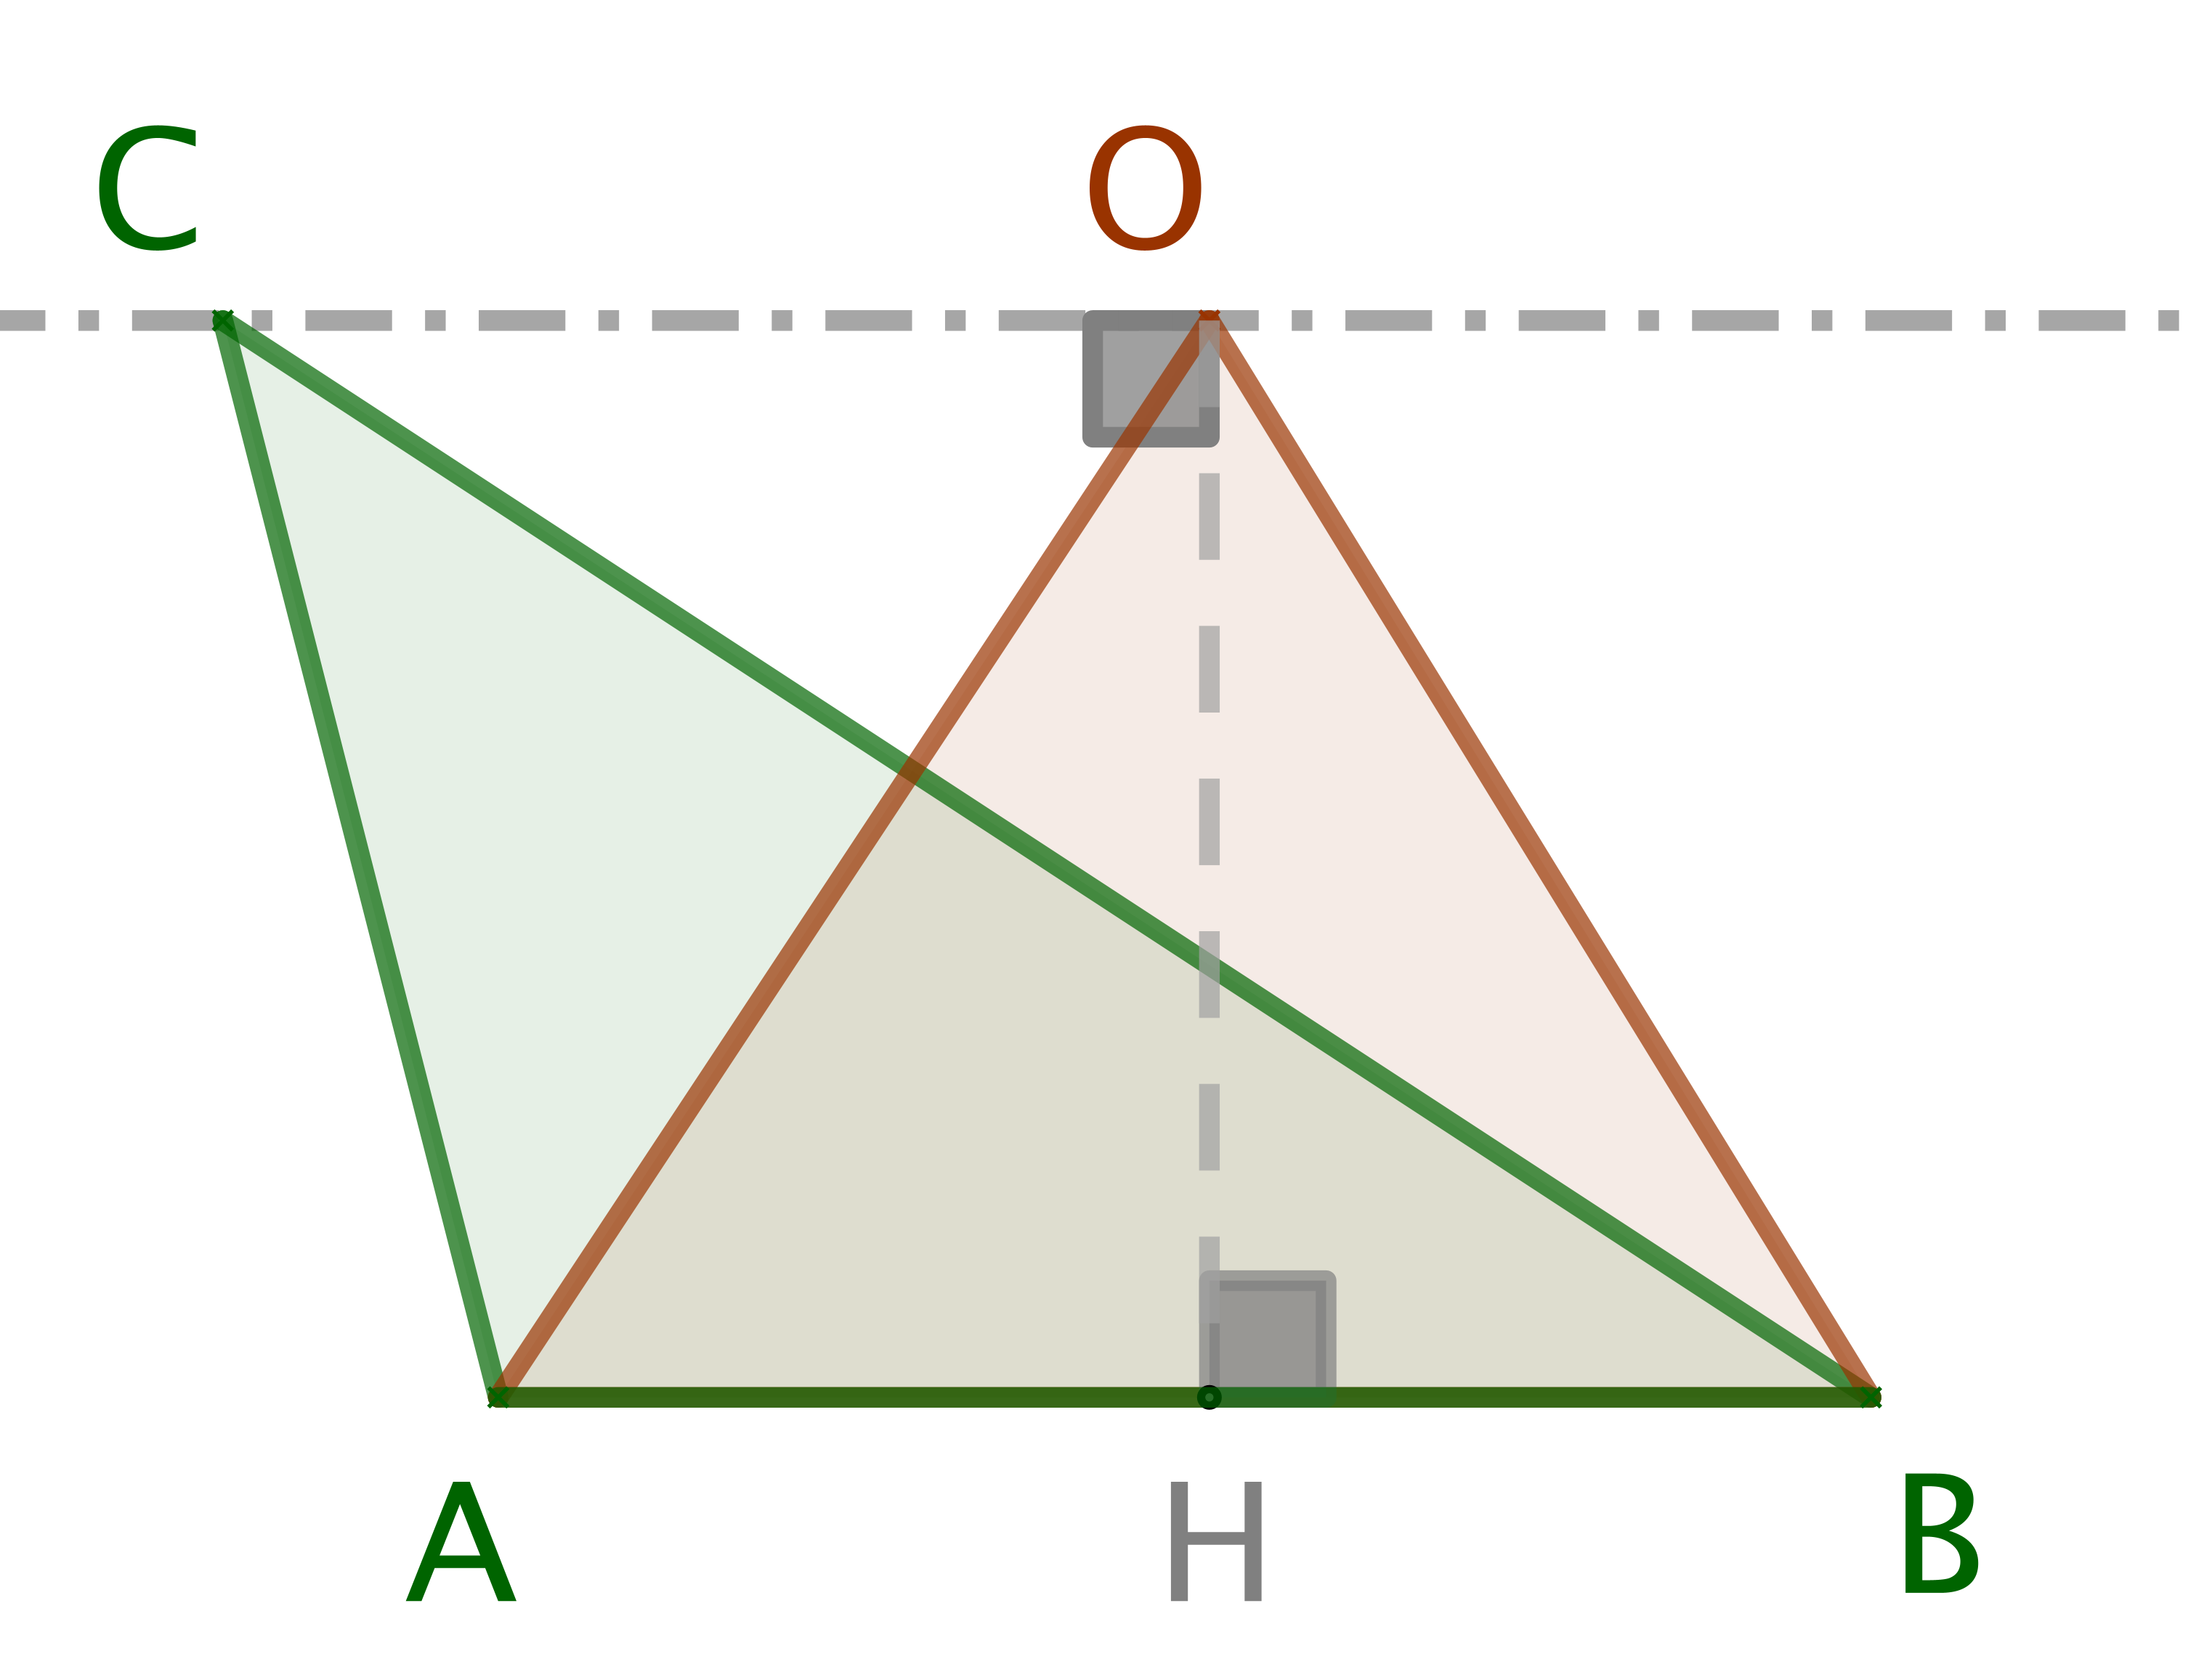
\includegraphics[scale=.4]{content/triangle-one-side-fixed/triangle.png}
	\end{center}

	
	Via une symétrie axiale, voir ci-dessous, il est aisé de noter que $\perim{ABC} \geq \perim{ABO}$, avec égalité uniquement si $ABC$ est isocèle en $C$.%
	\footnote{
		Plus précisément, en passant de $C$ à $O$, le périmètre diminue.
	}
	
	\begin{center}
		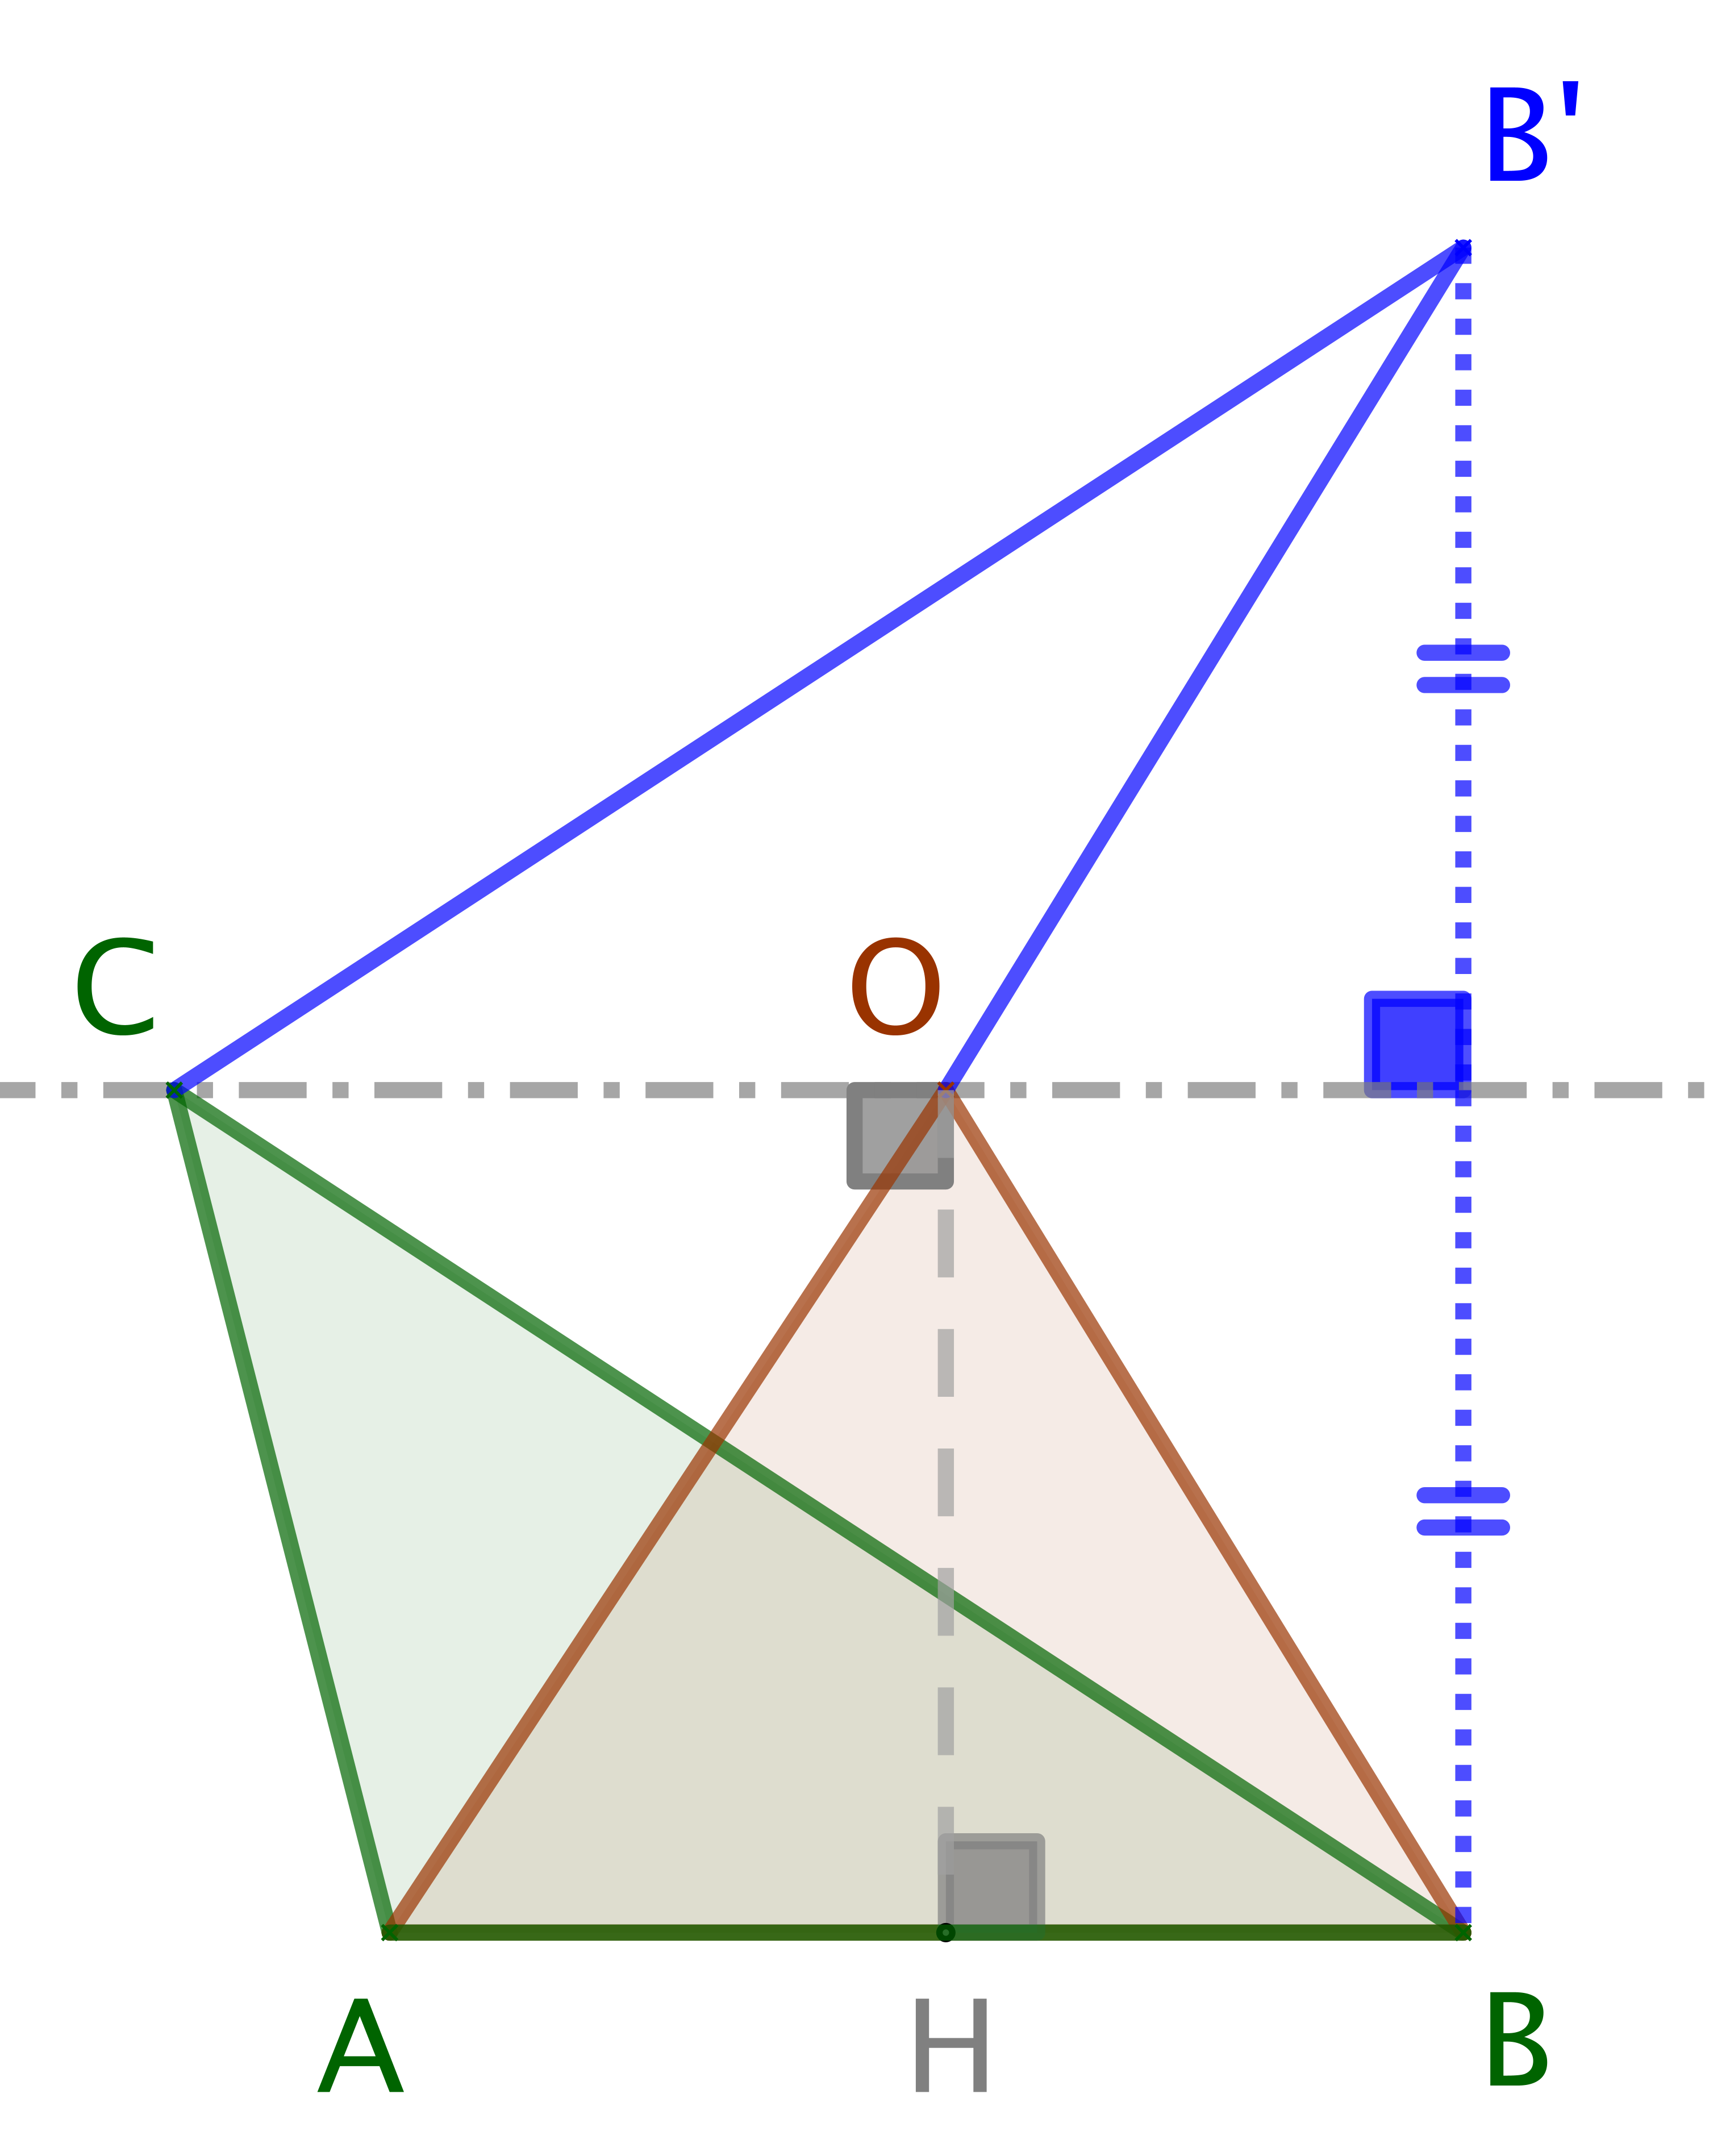
\includegraphics[scale=.4]{content/triangle-one-side-fixed/proof.png}
	\end{center}
	
	Une dilatation \og \emph{verticale} \fg\ de rapport $r = \frac{\perim{ABC}}{\perim{ABO}} \geq 1$ donne un triangle isocèle $ABO^{\,\prime}$ tel que 
	$\perim{ABO^{\,\prime}} = p$
	et 
	$\area{ABO^{\,\prime}} \geq \area{ABC}$, avec égalité uniquement si $ABC$ est isocèle en $C$. 
	Contrat rempli!%
	\footnote{
		La remarque \ref{constrained-extrema} explique comment employer la méthode des extrema liés. 
		Les arguments fournis à cet endroit s'adaptent facilement au cas des triangles de base fixée.
	}
\end{proof}


% ----------------------- %


\begin{remark}
	La recherche parmi les triangles avec un côté fixé de celui ayant un périmètre minimal pour une aire fixée est le problème dual de l'isopérimétrie pour ces triangles.
\end{remark}
